\section{Results and Discussion}

\begin{figure}[h!]
    \centering
    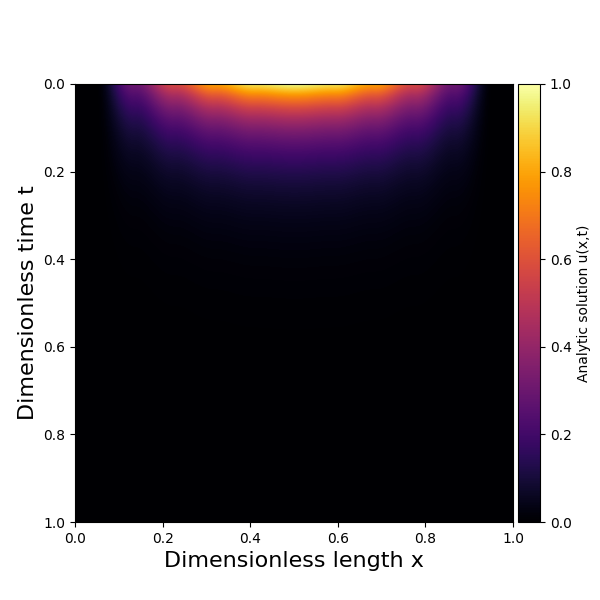
\includegraphics[width=8cm]{../Figures/analytic_solution.png}
    \caption{Analytic solution for the heat equation with initial conditions
    $u(x,0)=\sin{(\pi x)}$ and boundary conditions $u(0,t)=u(1,t)=0$.}
    \label{fig:analytic_solution}
\end{figure}

\textit{All networks are initialized with weights drawn from a Xavier uniform
initializer and bias=0}.
\\~\\
In figure \ref{fig:analytic_solution} we see the analytic solution for our
given boundary and initial conditions. This will be used to test our numerical
solvers using the absolute error between this and the numerical approximation.
This can be seen in figure \ref{fig:abs_error_all}. In the subfigures (a)-(d)
we see the NNs prediction for different activation functions and optimizers. We
can see that ReLu with RMSprop has the lowest error. And we note that all of
the approximations have the highest loss at the boundaries. We can especially
see that Adam with ReLu has a very high error at the $t=0$ boundary. The reason
our network is not handling the boundaries well is because the loss function
has no special penalizing of wrong boundaries. This could be fixed by creating
a new loss function by looking at the minimization of the NNs prediction

\begin{equation*}
    \min_{\hat{u}} \left\{
    \lVert \hat u_{xx} - \hat u_t \rVert^2 
    + \lVert \hat u(0,t) \rVert^2 
    + \lVert \hat u(1,t) \rVert^2
    + \lVert \hat u(x,0)-\sin{(\pi x)}\rVert^2 \right\},
\end{equation*}
where this norm $\lVert \cdot \rVert$ is to be read as the grand sum of the
matrix. We then define our cost/loss-function as
\begin{equation*}
    C(\hat u) =\frac{1}{2} \left[ \lVert \hat u_{xx} - \hat u_t \rVert^2 
    + \lVert \hat u(0,t) \rVert^2 
    + \lVert \hat u(1,t) \rVert^2
    + \lVert \hat u(x,0)-\sin{(\pi x)}\rVert^2 \right].
\end{equation*}
We can then add parameters in front of the norms to decide how costly it would
be for the network to not prioritize the boundaries. This is called a physics
informed neural network and has been explored in a previous paper (Zobeiry \&
Humfeld, 2020)\cite{2}. Getting back to figure \ref{fig:abs_error_all}, we look
at the explicit solver in (e). Note here that the limits on the colorbar is
changed because the error is so small compared to that of the NNs. We see that
now our boundaries is forced to be correct. And we can see that as we move in
time the middle of the rod gets a larger and larger error until it starts
cooling down and of course the error gets smaller because the values get closer
and closer to zero because of the $u(0,t)=u(1,t)=0$ boundaries. We look more at
the explicit solver in \ref{fig:MSE_b}. We can see a big drop in MSE as half
$\alpha$ from the criterion $1/2$ to $1/4$. By doing this we decrease the MSE
by about 4 orders of magnitude. While decreasing $\Delta x$ by $10$ we only get
a decrease in MSE of about one order of magnitude. This means that decreasing
$\alpha$ will have the biggest effect on the accuracy of the solution. Now
looking at \ref{fig:loss_vs_epochs} we can see loss versus epochs for different
activation functions and optimizers. We see that the MSE is higher for all of
these compared to the explicit solver. And we see that Adam with ReLu looks
constant. This could be because the network died or it reaches a local minima
in the gradient decent.



\begin{figure}[h!]
    \centering
    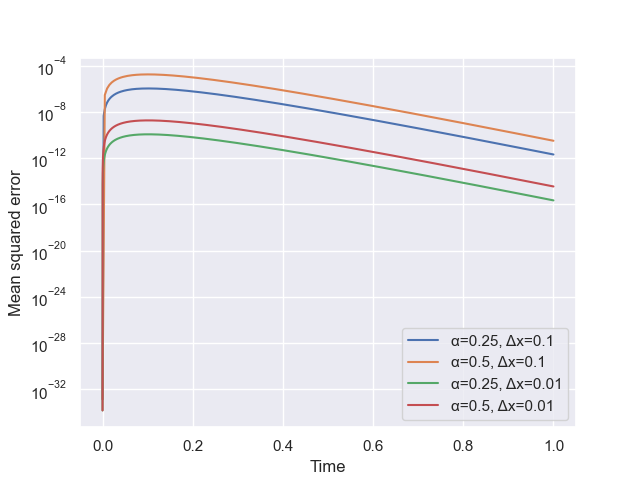
\includegraphics[width=8cm]{../Figures/b_mse.png}
    \caption{MSE of explicit solver for different $\alpha=\Delta t/\Delta x^2$
    and $\Delta x$ values.}
    \label{fig:MSE_b}
\end{figure}

\begin{figure}[h!]
    \centering
    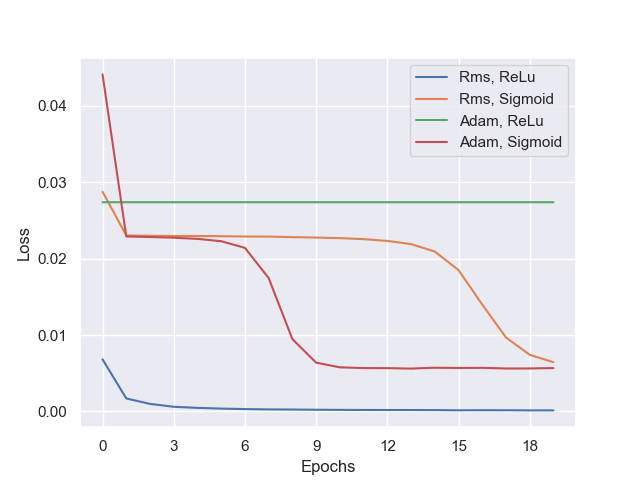
\includegraphics[width=8cm]{../Figures/loss_vs_epochs.png}
    \caption{MSE loss function for different optimizers and activation functions.
    All are run with a batch size of 30 and trained on a $(n=100)\times
    (m=100)$ matrix against the analytical solution. The networks have 3 hidden
    layers, one of 16 neurons and two of 32 neurons.}
    \label{fig:loss_vs_epochs}
\end{figure}

We further explore RMSprop with ReLu since this has the lowest MSE. In figure
\ref{fig:loss_vs_layers} we see the MSE as a function of epochs for different
number of hidden layers. We see that for 5 hidden layers we have a constant
loss. This could be because the network is too complex for our problem and
dies. This may be solved with different initializations of weights and biases.
But it seems like for 3 and 4 hidden layers we do not get a big difference in
MSE so 3 hidden layers may be enough for such a simple problem. 

\begin{figure}[h!]
    \centering
    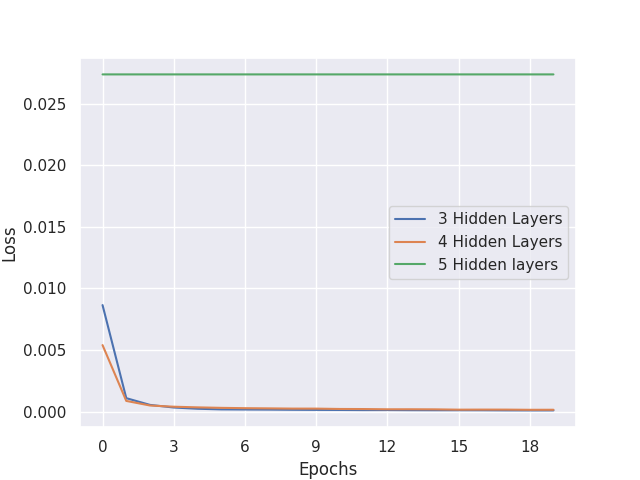
\includegraphics[width=8cm]{../Figures/loss_vs_layers.png}
    \caption{MSE loss function for different number of hidden layers. First
    hidden layer is 16 neurons and the rest are 32. 
    All are run with a batch size of 30 and trained on a $(n=100)\times
    (m=100)$ matrix against the analytical solution. Activation functions and
    ReLu and the optimizer is RMSprop.}
    \label{fig:loss_vs_layers}
\end{figure}

We chose our 3 layer network with RMSprop activation function and Adam
optimizer and train this. Then in figure \ref{fig:time_vs_size} we see the time it takes to
predict depending on the matrix size against the time used by the explicit
solver. We can see that in logspace both graphs are linear, meaning they are
taking exponentially more time as we increase the matrix size. This is
expected for the explicit solver. For the Neural Network we disregard the low
matrix size points because this is only run one time and is therefore very
dependent on small variations by the processes already running on the computer.
These effects will be smaller and smaller the bigger the matrix size as such
effects will average out. So then we can also say that the predictions of the
neural networks grow linearly in logspace. And it is about two orders of
magnitude bigger than the explicit solver.

\begin{figure}[h!]
    \centering
    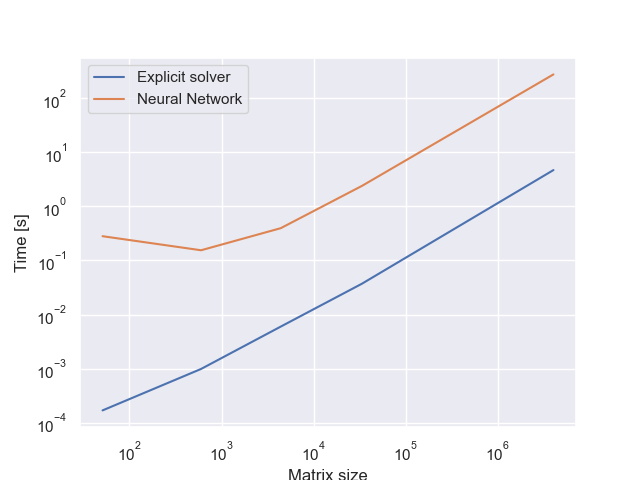
\includegraphics[width=8cm]{../Figures/time_vs_matrix_size.png}
    \caption{Time vs matrix size for a neural network with three hidden layers,
    one of 16 neurons and two of 32 neurons. The network is already trained
    using a batch size of 30 on a $(n=100)\times
    (m=100)$ matrix against the analytical solution. Activation functions and
    ReLu and the optimizer is RMSprop. And the explicit solver has $\alpha=1/4$
    and uses different $\Delta x$ to calculate the matrix size that the NN gets
    to solve. Run on a 1,8 GHz dual-core Intel Core i5.}
    \label{fig:time_vs_size}
\end{figure}

\begin{comment}
\begin{figure}
\centering
\subfigure[Rms, ReLu]{\label{fig:a}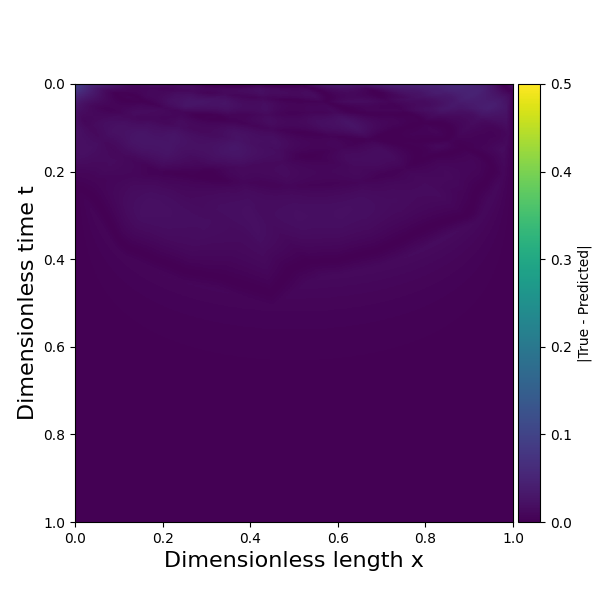
\includegraphics[width=70mm]{../Figures/error_rms_relu.png}}
\subfigure[Rms, Sigmoid]{\label{fig:b}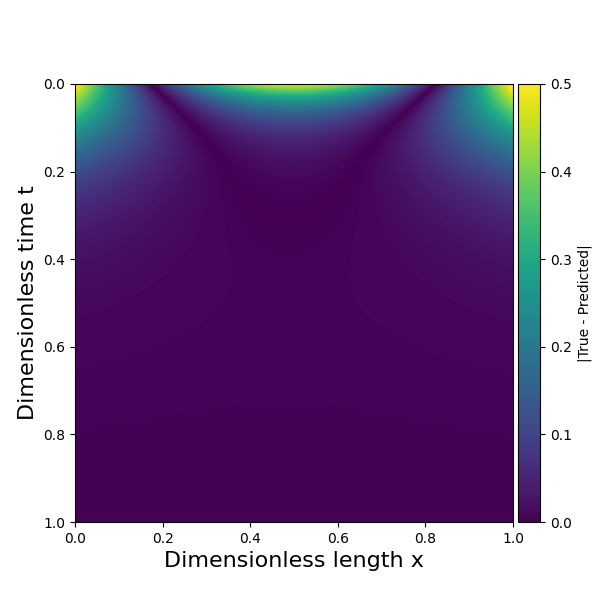
\includegraphics[width=70mm]{../Figures/error_rms_sigmoid.png}}
\subfigure[Adam, ReLu]{\label{fig:c}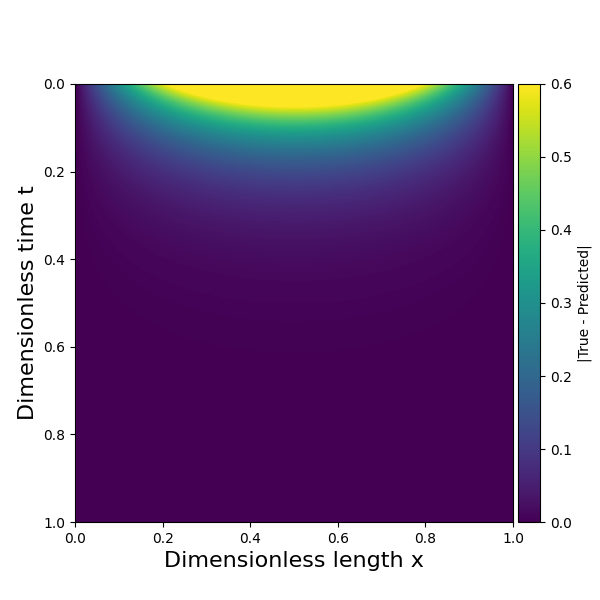
\includegraphics[width=70mm]{../Figures/error_adam_relu.png}}
\subfigure[Adam, Sigmoid]{\label{fig:d}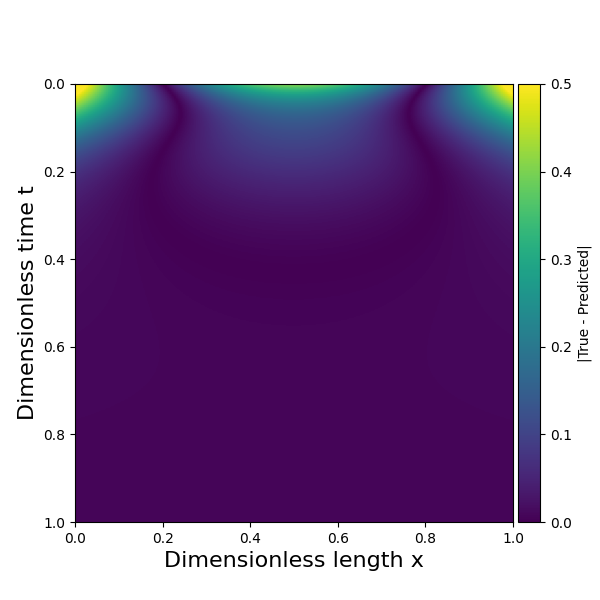
\includegraphics[width=70mm]{../Figures/error_adam_sigmoid.png}}
\subfigure[Explicit solver]{\label{fig:e}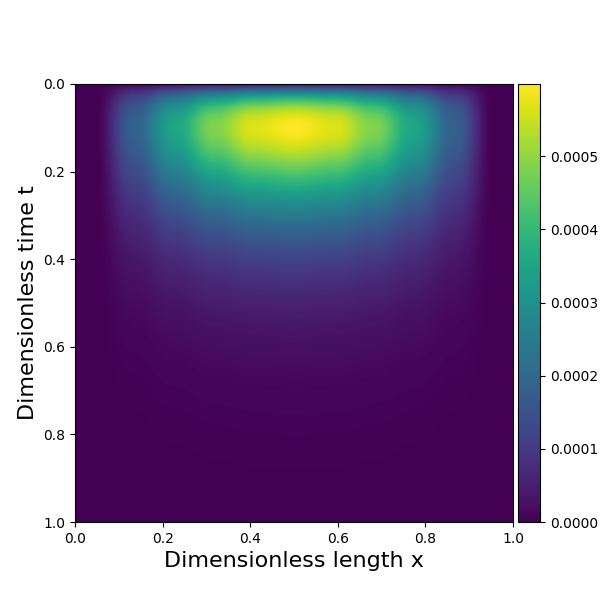
\includegraphics[width=70mm]{../Figures/error_explicit.png}}
\caption{Absolute error for NN in (a)-(d) and explicit solver in (e). NN is
trained with 20 epochs and a batch size of 30 with $(n=100)\times (m=100)$
data points of $x$
and $t$ respectively, using the analytical solution for MSE as the loss
function. The networks have three hidden layers, one of 16 neurons and two of 32.
The explicit solver in (e) is using $\Delta x=0.1$ and $\alpha=1/4$.}
\label{fig:abs_error_all}
\end{figure}
\end{comment}


